\documentclass[10pt]{IEEEtran}

\usepackage{listings}
\usepackage[USenglish]{babel}
\usepackage{graphicx} % figuras
\usepackage{subfigure} % subfigura
\usepackage[utf8]{inputenc}
\usepackage{cite} 
\usepackage{hyperref}
\usepackage{algpseudocode}
%\usepackage[dvips]{graphicx}



\title{Tarea 1. Detección de líneas de carril en autopista }

\author{Miguel Mendoza}
\newcounter{neq}
\begin{document}

\maketitle

\section{Introducci\'on}
Encontrar señales de tránsito como son las líneas divisoras de carril en las autpistas es un labor sencilla para el ser humano, sin embargo, cuando se requiere obtener dicha información de forma autónoma con un sensor de adquisición de imágenes se convierte en una tarea de grandes retos.\\
Se presenta el desarrollo de un proyecto para la detección de líneas de tránsito en un carril sobre una autopista. Se lleva a cabo el procesamiento sobre una imagen y también sobre videos con distintos elementos comunes en situaciones reales que influyen significativamente para obtener resultados correctos.


\section{Desarrollo}
El procesamiento se realizó usando librerías de OpenCV sobre la imágen mostrada en la imagen \ref{fig:exit_ramp} y en tres videos grabados con una cámara montada al frente de un automóvil, dos de los videos presentan un ambiente sin perturbaciones como son sombras y distintas intensidades de iluminación debido a la luz del sol, y otro de los videos presenta estás perturbaciones que son elementos comunes en una situación real. 

\section{Algoritmo}
Se enuncia el algoritmo para encontrar las líneas del carril en la imagen \ref{fig:exit_ramp}:\\

\begin{algorithmic}[1]
\State Lectura de imagen de entrada
\State Transformación a escala de grises.
\State Aplicación de filtro de Canny.
\State Aplicación de filtro Gaussiano.
\State Definición de una máscara sobre las regiones de interés de la imagen, en éste caso son los carriles.
\State Aplicación de transformada de Hough sobre las regiones de interés.
\State Definición de pendiente mínima, pendiente máxima, cont izq, cont der, pend izq, pend der, intersección izq y intersección der.	
\For {línea inicial de Hough \textit {hasta} línea final de Hough}
	\State{Calcular pendiente}
	\If { x1 = x2 \textbf{and} y1 = y2}
		\State continuar
	\ElsIf { pendiente minima $<$ pendiente $<$ pendiente máxima}
		\State Calcular intercepción (valor $b$ de la recta)
			\If { pendiente $<$ 0}
				\State  Contador izq + 1 $\rightarrow$  contador izq
				\State Pendiente izq + pendiente $\rightarrow$ pendiente izq 
				\State Intersección izq + intersección $\rightarrow$  intersección izq
			\Else
				\State Contador der + 1 $\rightarrow$  contador der
				\State Pendiente der + pendiente $\rightarrow$ pendiente der
				\State Intersección der + intersección $\rightarrow$ intersección der
			\EndIf
	\EndIf
\EndFor
\State Pendiente izq / contador izq$\rightarrow$ pendiente izq
\State Intersección izq / contador izq$\rightarrow$ intersección izq
\State Pendiente der / contador der$\rightarrow$ pendiente der
\State Intersección der / contador der$\rightarrow$ intersección der
\State Definir $y_{1}$ del 60 $\%$ de los renglones totales de la imagen
\State Definir $y_{2}$ del 60 $\%$ de los renglones totales de la imagen
\State ($y_{1}$ - intersección izq) / pendiente izq $\rightarrow$ $x_{1}$
\State ($y_{2}$ - intersección izq) / pendiente izq $\rightarrow$ $x_{2}$
\State Trazar línea sobre imagen original de entrada
\State ($y_{1}$ - intersección der) / pendiente der $\rightarrow$ $x_{1}$
\State ($y_{2}$ - intersección der) / pendiente der $\rightarrow$ $x_{2}$
\State Trazar línea sobre imagen original de entrada
\State Mostrar Imagen de salida con líneas detectadas
\end{algorithmic}

Para el caso del algoritmo usado en los videos se realizó la modificación de acuaerdo a los comandos de OpenCV \cite{opencvvideo} de leer la imagen por cada frame del video y al final se guarda el video.

\section{Resultados}
Los resultados obtenidos se muestran en las imágenes \ref{fig:grises}, \ref{fig:bordes}, \ref{fig:bordes_region}, \ref{fig:mascara}, \ref{fig:hough_region} y \ref{fig:final}, donde la imagen \ref{fig:grises} es el resultado de aplicar la transformación de escala de grises y filtro gaussiano a la imagen \ref{fig:exit_ramp}. La imagen \ref{fig:bordes} muestra la salida de la imagen \ref{fig:grises} después de haber aplicado filtro de canny. Después se aplica la máscara mostrada en la imagen \ref{fig:mascara} a la imagen \ref{fig:bordes}, el procesamiento de las operaciones restantes se realizan solamente sobre ésta región obteniendo la imagen \ref{fig:bordes_region} y posteriormente se muestra en la imagen \ref{fig:hough_region} las líneas encontradas usando Hough y por último se muestra la imagen \ref{fig:final} con las líneas finales detectadas sobre la imagen inicial.\\
La imagen \ref{fig:exit_ramp} es una imagen fácil de procesar y obtener buenos resultados ya que no existe ruido o perturbaciones que afecten a los filtros aplicados a diferencia de los videos. El código se encuentra disponible en la liga \url{https://github.com/MiguelMendozaG/Vision-3d/blob/master/lineas_video.py}


\section{Conclusion}
Los resultados obtenidos fueron buenos ya que en los videos se observa un buen comportamiento de las lineas. Se encontró un problema analizando los resultados de dos videos, uno de ellos con perturbaciones y el otro en buenas condiciones, se considera que controlando la distancia de la cámara de tal forma que los carriles entren en un rango de los pixeles entonces la máscara puede reducirse de tal forma que filtre las regiones más importantes de la imagen. Las perturbaciones de las sombras y cambios de intensidad de la luz generan que las lineas sean promediadas con ruido ocasionando que las líneas encontradas no sean pintadas correctamente. Se visualizan otros casos en los que evidentemente se tendran problemas, como por mencionar algunos: cuando un objeto entre en el campo de visión entre los carriles o cuando las líneas no estén perfectamente pintadas.

\begin{figure}[h]
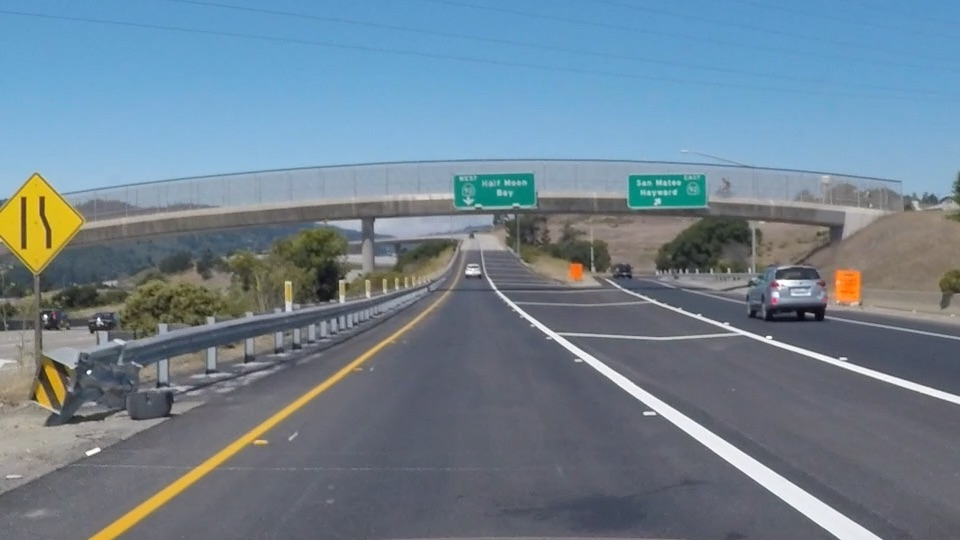
\includegraphics[scale = 0.25]{exit_ramp.jpg}
\caption{Escena principal}
\label{fig:exit_ramp}
\end{figure}

\begin{figure}
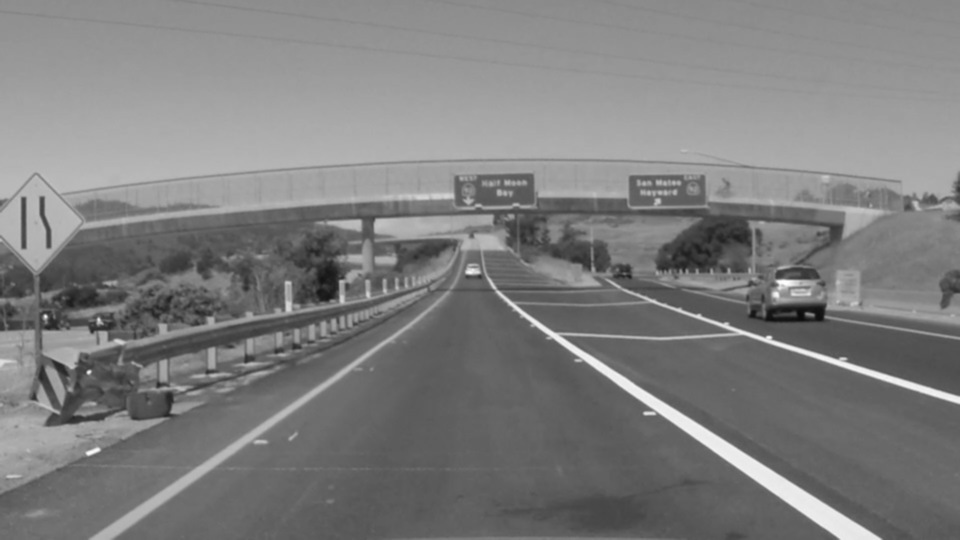
\includegraphics[scale = 0.25]{grises.png}
\caption{Filtro gaussiano y de canny}
\label{fig:grises}
\end{figure}

\begin{figure}
\includegraphics[scale = 0.25]{bordes.png}
\caption{Bordes}
\label{fig:bordes}
\end{figure}

\begin{figure}
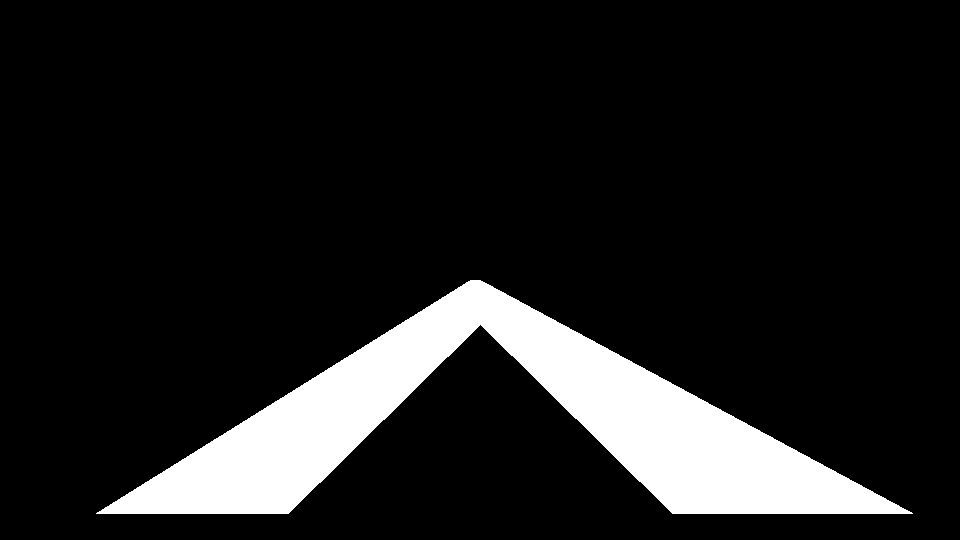
\includegraphics[scale = 0.25]{mascara.png}
\caption{Máscara sobre región de interés}
\label{fig:mascara}
\end{figure}

\begin{figure}
\includegraphics[scale = 0.25]{bordes_region.png}
\caption{Bordes en región de interés}
\label{fig:bordes_region}
\end{figure}

\begin{figure}
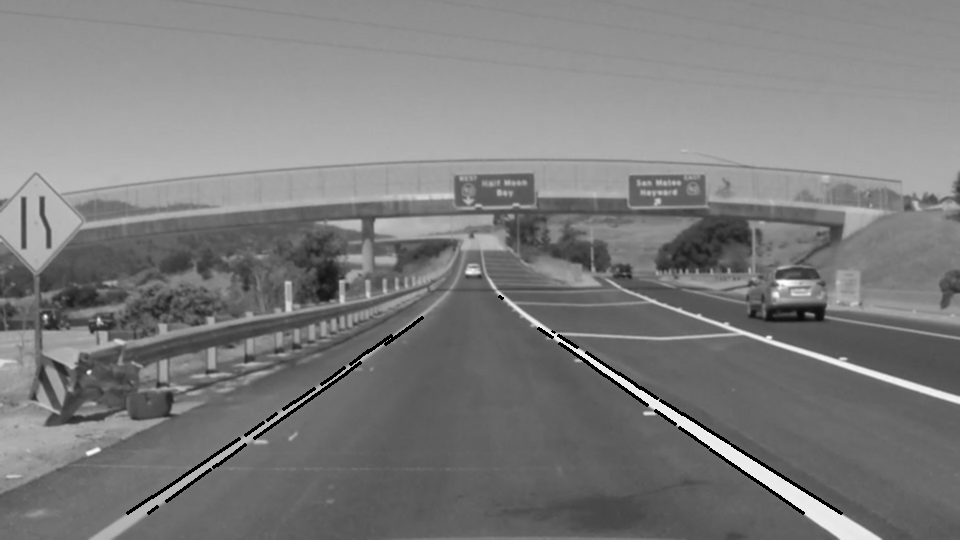
\includegraphics[scale = 0.25]{hough_region.png}
\caption{Líneas de Hough en región de interés}
\label{fig:hough_region}
\end{figure}

\begin{figure}
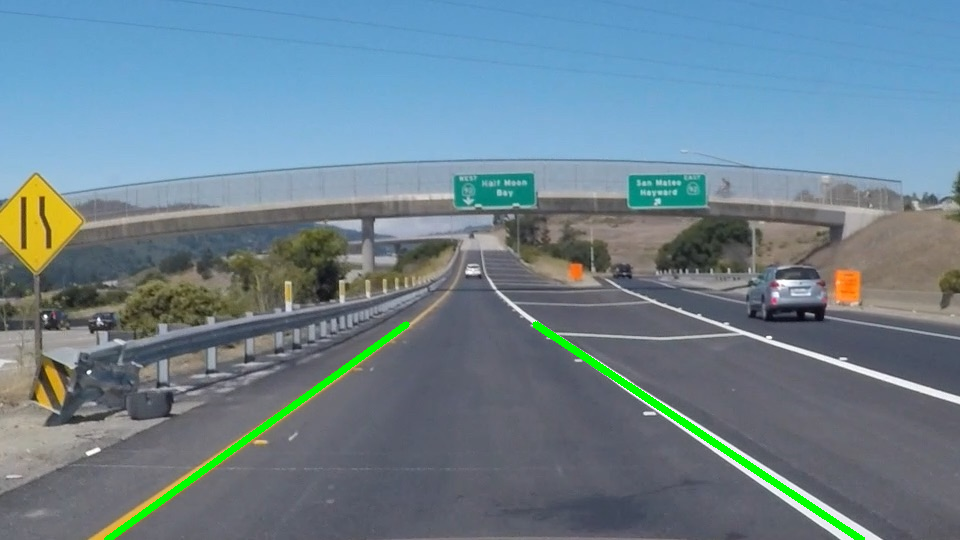
\includegraphics[scale = 0.25]{final.png}
\caption{Líneas detectadas}
\label{fig:final}
\end{figure}

\bibliographystyle{acm}
\bibliography{tarea1}

\end{document}